
\section{Results}
\begin{figure}
  \setlength{\unitlength}{\textwidth}
  \begin{picture}(1,0.72)
%(0,0.35)
    
    % % %Parkinson Data 
    \put(0.025,0.48){\includegraphics[width=0.5\unitlength]{../FnP/gnuplot/displacement_amp_re_parkinson_1.eps}}
    \put(0.025,0.25){\includegraphics[width=0.5\unitlength]{../FnP/gnuplot/velocity_amp_re_parkinson.eps}}
    \put(0.025,0.02){\includegraphics[width=0.5\unitlength]{../FnP/gnuplot/mean_power_re_parkinson.eps}}
    
    % Re 165 Data 
    \put(0.495,0.48){\includegraphics[width=0.5\unitlength]{../FnP/gnuplot/displacement_amp_re165.eps}}
    \put(0.495,0.25){\includegraphics[width=0.5\unitlength]{../FnP/gnuplot/velocity_amp_re165.eps}}
    \put(0.495,0.02){\includegraphics[width=0.5\unitlength]{../FnP/gnuplot/mean_power_re_165.eps}}
   
%    \put(0.25,0.93){\ustar}
%    \put(0.8,0.93){\ustar}
%    \put(0.25,0.63){\ustar}
%   \put(0.8,0.63){\ustar}
    \put(0.25,0.0){\ustar}
    \put(0.75,0.0){\ustar}
    
    \put(0.00,0.685){$\frac{A}{D}$}
%    \put(0.52,1.075){$\frac{A}{D}$}
    \put(0.00,0.44){$\frac{V}{D}$}
%    \put(0.52,0.83){$\frac{V}{D}$}
    \put(-0.01,0.15){$\frac{P_{m}}{\rho \mathcal{A}U^3 }$}
%    \put(0.5,0.54){$\frac{P_{m}}{\rho \mathcal{A}U^3 }$}
    
    \put(0.095,0.685){\small(a)}
    \put(0.555,0.685){\small(b)}
    \put(0.095,0.455){\small(c)}
    \put(0.555,0.455){\small(d)}
    \put(0.095,0.225){\small(e)}
    \put(0.555,0.225){\small(f)}   
  \end{picture}

%  \vspace{-4cm}
  \caption{Velocity and displacement amplitude and mean power  as a function of $U^*$. (a), (c) and (e) are calculated using input $C_y$ data at Re=22300 obtained by \cite{Parkinson1964} and present data at three different damping ratios: $\zeta=0.0125$ (\ding{83}), $\zeta=0.015$ (\ding{116}) and $\zeta=0.0175$ (\ding{108}). (b),(d) and (f) are from $C_y$ data at Re=165 and are calculated  from the fixed body simulations and present data at three different  different damping ratios: $\zeta=0.075$ ($\times$), $\zeta=0.1$ (\ding{117}) and $\zeta=0.15$ (+). The multiple branches for the higher Re are due to the hysteresis between two solutions.}
  
  \label{fig:uncollapsed_data}
\end{figure}



\subsection{Displacement,velocity and power output as a function of reduced velocity}


 The quasi-steady analysis data reveals that the displacement amplitude tend to grow with increasing $U^*$ Fig.\ref{fig:uncollapsed_data} (a) and (b). The onset of galloping is delayed with increasing $\zeta$ for both high and low Reynolds numbers. This echo the findings of previous studies \cite{Parkinson1964} and \cite{Barrero-Gil2010a}. Hysteresis could be observed at higher Reynolds numbers. 

 
 \subsubsection*{Power vs $U^*$}
 
 The mean power grows, peaks and then reduces as $U^*$ is increased (Fig.\ref{fig:uncollapsed_data} (e) and (f)) for each value of $\zeta$. A shift of the peak power could be observed as $\zeta$ increases. However, the magnitude of the peaks remain constant for all the values of $\zeta$. A similar observation could be made from the results of \cite{Barrero-Gil2010a}. It could be observed that unlike VIV the  system has no preferred frequency. The onset of galloping and the peak power occurs at different $U^*$ at when the damping ratio is changed. The peak power remains constant regardless of $U^*$.
 
 \subsection{Galloping response and natural frequency}
 
 If the oscillator equation Eq.\eqref{final_equation_motion} is considered from a power perspective (disregarding the shedding term as the net effect is negligible !!! this should be elaborated further possibly in an earlier section as to why. I suggest when you talk about this when you discuss the shedding parameters and discuss the findings from Joel. 
 
 Only negligible when system oscillates at natural frequency which is far from shedding frequency), it could be seen that the forcing term on RHS of the equation is only dependent on transverse velocity($\dot{y}$) which is essentially the input power of the system. On the RHS, the mechanical damping or system damping is the only term that takes out power at any instant by the product of damping force and the velocity ($P_d$). The inertia and the stiffness terms governs the frequency of the system but the forces associated by those terms are conservative forces i.e there is zero net energy in or out of the system when averaged over a period. Therefore it appears that the system is governed by the transverse velocity rather than the natural frequency.
 

 Using $U^*$ and $\zeta$ assumes that the system has a preferred frequency. The effect of fixing $\zeta$ and increasing $U^*$ actually decreases damping constant for a fixed free-stream velocity.($U^*=\frac{U}{f \times D}$, $\zeta= \frac{c}{2 m \omega_n}$ ). Both these effects leads to the multiple lines that are horizontally transpose when $\zeta$ is increased(Fig.\ref{fig:uncollapsed_data} (e) and (f)). Therefore the effect of $\zeta$ essentially scales up the damping coefficient for a fixed $U^*$. 
 \vspace{1cm}
 
 Therefore a single set of results for a given instantaneous lift ($C_y$) could be obtained if we were to plot displacement, velocity and power as a function of damping constant $c$ (Fig \ref{fig:velocity_collapsed}, \ref{fig:meanpower_collapsed}). A similar maximum velocity could be obtained for a given `c'. Fig.\ref{fig:same_max_vel} clearly shows the validity of this argument. 
 

\begin{figure}
  \setlength{\unitlength}{\textwidth}
       
        \begin{picture}(1,0.52)

      % % % Parkinson Data 
      \put(0.025,0.27){\includegraphics[width=0.5\unitlength]{../FnP/gnuplot/velocity_amp_collapsed_parkinson.eps}}
      \put(0.495,0.27){\includegraphics[width=0.5\unitlength]{../FnP/gnuplot/velocity_amp_collapsed_re165.eps}}
      
      \put(0.025,0.02){\includegraphics[width=0.5\unitlength]{../FnP/gnuplot/mean_power_collapsed_parkinson.eps}}
      \put(0.495,0.02){\includegraphics[width=0.5\unitlength]{../FnP/gnuplot/mean_power_collapsed_re_165.eps}}
      
      
      \put(0.23,0.00){ $c\rho\mathcal{A}U$}
      \put(0.73,0.00){ $c\rho\mathcal{A}U$}
      
      \put(0.01,0.405){$\frac{V}{D}$}
      
      \put(0,0.13){$\frac{P_{m}}{\rho \mathcal{A}U^3 }$}
      \put(0.085,0.475){\small(a)}
      \put(0.555,0.475){\small(b)}
      \put(0.095,0.225){\small(c)}
      \put(0.555,0.225){\small(d)}
      
    \end{picture}

  \caption{ Velocity amplitude and mean power  as a function of $c$ (damping constant). (a) and (c)  are calculated using input $C_y$ data at Re=22300 obtained by \cite{Parkinson1964} and present data at three different damping ratios: $\zeta=0.0125$ (\ding{83}), $\zeta=0.015$ (\ding{116}) and $\zeta=0.0175$ (\ding{108}). (b)and (d)  are at Re=165 are calculated  from the fixed body simulations and present data from three different damping ratios: $\zeta=0.075$ ($\times$), $\zeta=0.1$ (\ding{117}) and $\zeta=0.15$ (+). The collapsed data implies that there is no frequency selection and the tuning parameter of the mechanical side of the system is the damping constant to obtain an optimum power output.}
    \label{fig:collpased_data}
\end{figure}

\ %vspace{10cm}

 
\begin{figure}
  \setlength{\unitlength}{\textwidth}
  \begin{picture}(1,0.3)(0,0.8)
    % % %90
    \put(0.025,0.83){\includegraphics[width=0.5\unitlength]{../FnP/gnuplot/vel_time_history_60_0.075.eps}}
    \put(0.495,0.83){\includegraphics[width=0.5\unitlength]{../FnP/gnuplot/vel_time_history_165_0.175.eps}}
    
    \put(0.03,0.95){ $\frac{V}{D}$} 	
    % \put(0.56,1.02){ $\frac{V}{D}$}
 	
    \put(0.25,0.805){ $\frac{tU}{D}$} 	
    \put(0.73,0.805){ $\frac{tU}{D}$}

    \put(0.095,1.03){(a)}
    \put(0.565,1.03){(b)}

  \end{picture}

  \caption{Time histories of velocity at two different $\zeta$ and $U^*$ which produce the same mean power ($1.2\times10^{-3}$). Data presented using QSS assumption, (a) at $\ustar=60$ and $\zeta=0.075$, (b) at $\ustar=165$ and $\zeta=0.175$ at Re=165. Shedding is evident in both signals as a high frequency fluctuation but the amplitude of the slower fluctuations remains constant in both cases.}
    \label{fig:time_hostory_velocity_same_power}
\end{figure}


 
 Power could be expressed as the product of force and velocity. Therefore the transferred power form fluid-to-body could be expressed as $P_t=F_y\dot{y}$. Similarly the dissipated power due to the mechanical damping could be expressed as $P_d=(c\dot{y})\dot{y}$. The time average of these two quantities should be equal when mechanical friction is neglected due to energy conservation. The analysis of time histories of $P_t $ and $P_d$ at key regions (Fig.\ref{fig:regions_1}) on the mean power vs $U^*$ provides a detailed explanation for the varying power output when the reduced velocity is increased. It has been established earlier that the damping factor is a function of $U^*$. It could be derived that $U^*$ is inversely proportional to damping coefficient. 

\begin{figure}[h!]
\centering
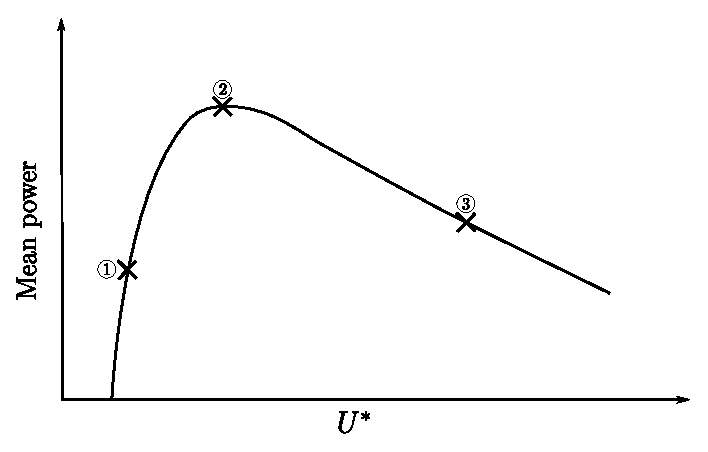
\includegraphics[width=0.5\textwidth]{../FnP/sketch_1}
\caption{ Three key regions taken into account to analyse the time histories of power in a typical the Mean power vs. $U^*$ curve at Re 165 }
\label{fig:regions_1}
\end{figure}


From Fig \ref{cy ploynomial} (a) shows that the instantaneous force rises until $4^0$ where it peaks and then falls and at round $6^0$ becomes negative. Maximum amount of power could be transferred within the peak region. At the region where the instantaneous force becomes negative it will be opposing the velocity $\dot{y}$.

$U^*=90$ (region 1) the damping constant is high and therefore a clear sinusoidal signal could be observed for both $P_d$ and $P_t$ Fig. \ref{fig:power_time_histories} (a). Fig.\ref{fig:power_time_histories} (d) and (g) shows that$\theta$ is in line or in phase with $F_y$. Hence both $P_d$ and $P_t$ becomes sinusoidal. However, due to the higher damping  $\theta$ does not go to the region where the peak power is produced.

At region 2 where the mean power output is at its maximum($U=165$), $P_t$ is not a pure sinusoidal signal. However, the  signal remains periodic. From the time history graph of $P_t$,two `peaks' are present in a single half cycle (Fig \ref{fig:power_time_histories} (b)). In this case at certain point in time $\theta$ arrives at the region where $F_y$ decreases but does not become negative when the angle is increased. Therefore, the force $F_y$ and $P_t$ reduces as the velocity further increases since $\theta = tan^{-1}(\frac{\dot{y}}{U})$. As the velocity $\dot{y}$ is sinusoidal, $\theta$ recovers back and this leads to two `peaks'  in a single half cycle.

At region 3 ($U^*= 400$) `$c$' is low in comparison with region 1 and 2 which leads to a low mean power output. From Fig.\ref{fig:power_time_histories} (c) .b $P_t$ becomes negative over some portion of the cycle. This is because $\theta$  passes the point where both $\theta$ and $c_y$ (therefore $c_y$) are positive. As the force opposes the direction of travel and the power becomes negative. On the other hand from an energy perspective we could see that the mechanical damping is not sufficient to dissipate out the energy transferred from the fluid to the structure during the part of the cycle when this occurs(as `$c$' is substantially low), therefore  part of this energy is transferred back to the fluid in the remaining part of the cycle.

 
  
\begin{figure}

  \setlength{\unitlength}{\textwidth}
 % \fbox{
  \begin{picture}(1,0.6)(0,0.35)
    
    % % %90
      \put(0.03,0.78){\includegraphics[width=0.35\unitlength]{../FnP/gnuplot/power_time_history_90.eps}}
      \put(0.03,.58){\includegraphics[width=0.35\unitlength]{../FnP/gnuplot/f_y_history_90.eps}}
      \put(0.03,0.4){\includegraphics[width=0.35\unitlength]{../FnP/gnuplot/theta_time_history_90.eps}}
      
      % %165
       \put(0.36,0.78){\includegraphics[width=0.35\unitlength]{../FnP/gnuplot/power_time_history_165.eps}}
       \put(0.36,.58){\includegraphics[width=0.35\unitlength]{../FnP/gnuplot/f_y_history_165.eps}}
       \put(0.36,0.4){\includegraphics[width=0.35\unitlength]{../FnP/gnuplot/theta_time_history_165.eps}}
       
       \put(0.68,0.78){\includegraphics[width=0.35\unitlength]{../FnP/gnuplot/power_time_history_400.eps}}
       \put(0.68,.58){\includegraphics[width=0.35\unitlength]{../FnP/gnuplot/f_y_history_400.eps}}
       \put(0.68,0.4){\includegraphics[width=0.35\unitlength]{../FnP/gnuplot/theta_time_history_400.eps}}
      
            
      
      
   
 	\put(0.55,0.36){\large $\frac{tU}{D}$}
 	\put(0.2,0.36){\large $\frac{tU}{D}$}
    \put(0.85,0.36){\large $\frac{tU}{D}$}
    
   
   	
   	\put(0.0,0.87){$\frac{P}{\rho \mathcal{A}U^3}$}
    \put(0.01,0.66){$F_y$}
    \put(0.01,0.49){$\theta$}
   	

    \put(0.08,0.78){(a)}
    \put(0.08,0.58){(d)}
    \put(0.08,0.38){(g)}
    
    \put(0.4,0.78){(b)}
    \put(0.4,0.58){(e)}
    \put(0.4,0.38){(h)}
    
    \put(0.72,0.78){(c)}
    \put(0.72,0.58){(f)}
    \put(0.72,0.38){(i)}
       
  \end{picture}
%}
  \caption{Time histories of $P_t$,$P_d$,$F_y$ and $\theta$ at $\ustar=90,165$ and $400$ where the mean power dissipated due to mechanical was calculated using equation \hilight{equation}. Data was obtained at $\zeta=0.1$ and $m^*=40$. The time histories of $P_t$ ( \solidrule[4mm]\hspace{1mm}) and $P_d$ (\protect\dashedrule) are presented in (a), (b) and (c) where \ustar is 90, 165 and 400 respectively.(d), (e) and (f) shows time histories of the instantaneous force $F_y$ and (g), (h) and (i) shows the time history of the instantaneous angle $\theta$ of the corresponding power plots above}
    \label{fig:power_time_histories}
\end{figure}





 



\subsection{Effect of $m^*$}

 \begin{figure}

  \setlength{\unitlength}{\textwidth}
  \begin{picture}(1,0.35)(0,0.7)
    
  \put(0.15,0.8){\includegraphics[width=0.7\unitlength]{../FnP/gnuplot/mean_power_collapsed_mstar.eps}}         
      
      
   
 	\put(0.11,1){\large $\frac{P_{m}}{\rho \mathcal{A}U^3 }$} 	

 	
 	 	\put(0.45,0.75){ $c\rho\mathcal{A}U$} 	
 	 

     

  \end{picture}

  \caption{Mean power as a function of damping factor.Data are presented at $m^*=10$ (\ding{108}), $m^*=20$ (\ding{83}), $m^*=40$ (\ding{115}), $m^*=60$ (+) at Re 165 and $\zeta=0.1$. The reduction of maximum mean power could be observed when $m^*<40$}
    \label{fig:m_star_mean_power}
\end{figure}

The maximum mean power at different $m^*$ Fig.\ref{fig:power_mstar_collapsed_165} was constant beyond $m^*=30$. However, at $m^* \leq 30$ an effect of $m^*$ it could be observed that the mean power curve reduces with $m^*$. This may be due to the fact that shedding dominates as the inertia of the system is reduced.  

!! Are you sure?? I am sure if you run cases without shedding you will still get less power. Shedding has very little influence when the galloping is sustained and the frequencies are far apart. I believe when m* is low, there is not enough inertia (stored kinetic energy in the first term of the oscillatory equation)  in the system to carry it over the cycle.
We could add a little value to this paper by investigating this a little further since everything is already set up. Turn off shedding and run at low m*. eg. M*=1 or 2. You will get nothing. So you cannot say shedding suppresses galloping. Galloping is suppressed by low m* and if there is no galloping then all you see is the response to shedding if shedding forces are present.
 !! 
 
 This was also reported by \cite{Joly2012} where an influence of vortex shedding was present on galloping amplitude at low mass ratios. 



 \begin{figure}
  \setlength{\unitlength}{\textwidth}

  \begin{picture}(1,1.13)(0,0)
    
    % % %90
      \put(0.25,0.78){\includegraphics[width=0.5\unitlength]{../FnP/gnuplot/fsi_displacement.eps}}
      \put(0.25,0.4){\includegraphics[width=0.5\unitlength]{../FnP/gnuplot/fsi_velocity.eps}}
      \put(0.25,0.025){\includegraphics[width=0.5\unitlength]{../FnP/gnuplot/fsi_power.eps}}
     
   
	
            
      
      
   
 	\put(0.25,0.98){ \large $\frac{A}{D}$} 	
 	\put(0.25,0.62){\large $\frac{V}{D}$}
 	\put(0.2,0.23){\large $\frac{P_{m}}{\rho \mathcal{A}U^3 }$}
 	
% 	 	\put(0.25,0.88){ \ustar} 	
% 	 	\put(0.8,0.88){ \ustar}
 	 	\put(0.5,0.0){ \ustar}



    \put(0.36,1.1){(a)}
    \put(0.34,0.72){(b)}
    \put(0.34,0.34){(c)}
   
       

  \end{picture}  
	
  \caption{Comparison of QSS (\ding{83}) and FSI (\ding{108}) data of displacement amplitude, velocity amplitude and mean power as a function of \ustar represented by (a), (b) and (c)respectively. Data were obtained at Re=165 and $\zeta=0.075$. An average error of $34\%$ could be observed for both displacement and velocity amplitude. Essential physics i.e the rise and fall of mean power could be captured of the FSI data}
    \label{fig:FSI_QSS_compare}
\end{figure}

\subsection{Comparsion with FSI simulations}
 Similar trends are captured for both displacement and velocity amplitudes between QSS and FSI simulations (Fig. \ref{fig:FSI_QSS_compare}(a) and \ref{fig:FSI_QSS_compare}(b)). Quantitatively a large discrepancy (average of $30\%$) could be observed between QSS and FSI data. Therefore the power also becomes significantly low (Fig.\ref{fig:FSI_QSS_compare}(c)). However, the FSI data (Fig.\ref{fig:FSI_QSS_compare} (c)) was able to produce the main the rise and the fall of mean power as $U^*$ is increased. The reasoning behind this the fact is that galloping is weak at Re 165  and therefore fluid damping has a significant effect. It was reported by \cite{Barrero-Gil2009} that galloping only starts to occur ar Re $\geq 159$. As power is function of $(\dot{y})^2$ the error between QSS and FSI power becomes significantly large.  
 
 Put conclusion here 
 
 

%\section{Conclusion}









 

 
 
 

 
 


 % % % % % % % % % % % % % % % % % % % % % % % % % % % % % % % % % % % % % % % % %

 
 
 
 
 
 
 
 
 
 
  
 
 